% !TeX spellcheck = en_GB
%%%% acra.tex

%\typeout{ACRA Instructions for Authors}

% This is the instructions for authors for ACRA.
\documentclass{article}
\usepackage{acra}
% The file acra.sty is the style file for ACRA. 
% The file named.sty contains macros for named citations as produced 
% by named.bst.

% The preparation of these files was supported by Schlumberger Palo Alto
% Research, AT\&T Bell Laboratories, and Morgan Kaufmann Publishers.
% Shirley Jowell, of Morgan Kaufmann Publishers, and Peter F.
% Patel-Schneider, of AT\&T Bell Laboratories collaborated on their
% preparation. 

% These instructions can be modified and used in other conferences as long
% as credit to the authors and supporting agencies is retained, this notice
% is not changed, and further modification or reuse is not restricted.
% Neither Shirley Jowell nor Peter F. Patel-Schneider can be listed as
% contacts for providing assistance without their prior permission.

% To use for other conferences, change references to files and the
% conference appropriate and use other authors, contacts, publishers, and
% organizations.
% Also change the deadline and address for returning papers and the length and
% page charge instructions.
% Put where the files are available in the appropriate places.


%%%%%%%%%%%%%%%%%%%%%%%%%%%%%%%%%%%%%%%%%%%%%%%%%%%%%%%%%%%%%%%%%%%%%%%%%%%%%%%%
% PACAKAGES
%%%%%%%%%%%%%%%%%%%%%%%%%%%%%%%%%%%%%%%%%%%%%%%%%%%%%%%%%%%%%%%%%%%%%%%%%%%%%%%%
\usepackage[pdftex]{graphicx}
\usepackage[math]{cellspace}
%\usepackage{textcomp}
%\usepackage{epstopdf}
\usepackage{natbib}
\usepackage{afterpage}
%\usepackage{hyperref}

%%%%%%%%%%%%%%%%%%%%%%%%%%%%%%%%%%%%%%%%%%%%%%%%%%%%%%%%%%%%%%%%%%%%%%%%%%%%%%%%
% #DEFINES
%%%%%%%%%%%%%%%%%%%%%%%%%%%%%%%%%%%%%%%%%%%%%%%%%%%%%%%%%%%%%%%%%%%%%%%%%%%%%%%%
% declare the path(s) where your graphic files are
\graphicspath{{./resources/}{./resources/tmp/}}
% and their extensions so you won't have to specify these with
% every instance of \includegraphics
\DeclareGraphicsExtensions{.pdf,.svg,.png}

% --> \cite command is treated as \citep (so as to be natbib compatible)
\let\cite\citep


%%%%%%%%%%%%%%%%%%%%%%%%%%%%%%%%%%%%%%%%%%%%%%%%%%%%%%%%%%%%%%%%%%%%%%%%%%%%%%%%
% TITLE & AUTHOR
%%%%%%%%%%%%%%%%%%%%%%%%%%%%%%%%%%%%%%%%%%%%%%%%%%%%%%%%%%%%%%%%%%%%%%%%%%%%%%%%
\title{A Parallelized \& Asynchronous Forward Simulation Framework to Inform Multi-Robot UAV Coordination via Akka Streams}
% Was: \title{Use of Akka Streams to Inform Forward Simulation in Robot Control}

\author{Peter B{\"o}hm\textsuperscript{1,2} and Surya P. N. Singh\textsuperscript{2}
\\ \textsuperscript{1}NextLogic, Brisbane, Australia
\\ \textsuperscript{2}The Robotics Design Lab, The University of Queensland, Brisbane, Australia
\\ {\texttt{peter@nextlogic.biz, spns@uq.edu.au}}}



%%%%%%%%%%%%%%%%%%%%%%%%%%%%%%%%%%%%%%%%%%%%%%%%%%%%%%%%%%%%%%%%%%%%%%%%%%%%%%%%
\begin{document}
\maketitle
%%%%%%%%%%%%%%%%%%%%%%%%%%%%%%%%%%%%%%%%%%%%%%%%%%%%%%%%%%%%%%%%%%%%%%%%%%%%%%%%

%%%%%%%%%%%%%%%%%%%%%%%%%%%%%%%%%%%%%%%%%%%%%%%%%%%%%%%%%%%%%%%%%%%%%%%%%%%%%%%%
% ABSTRACT
%%%%%%%%%%%%%%%%%%%%%%%%%%%%%%%%%%%%%%%%%%%%%%%%%%%%%%%%%%%%%%%%%%%%%%%%%%%%%%%%
\begin{abstract}
The essence of many approaches for solving and optimizing stochastic control process, such as those that arise in multi-robot coordinated operations, is to consider many candidate policies and select the best one.  For many dynamic robots, this in turn requires a huge number of forward simulations, especially when the model is complex.

We investigate the use of Akka Streams to parallelize robot simulation. This allows for asynchronous processing of data streams generated by multiple sensors on multiple robots in situations where it is not possible to pause the simulation during calculations or (network) communication. 
%At the same time, it encapsulates entire simulation into a self-contained set of processes. This, in turn, allows for multiple cases to be run in parallel.
% This is seen in stochastic multirobot optimization and control problems solved using reinforced learning (RL). 
%The use of Akka Streams 
This structure helps mitigate the effects of latency and provides an expressive DSL (Domain Specific Language) to define the stream transformation graphs.  It also helps reduce coordination errors and improve overall distributed simulation stability.  
\end{abstract}


%%%%%%%%%%%%%%%%%%%%%%%%%%%%%%%%%%%%%%%%%%%%%%%%%%%%%%%%%%%%%%%%%%%%%%%%%%%%%%%%
% INTRODUCTION
%%%%%%%%%%%%%%%%%%%%%%%%%%%%%%%%%%%%%%%%%%%%%%%%%%%%%%%%%%%%%%%%%%%%%%%%%%%%%%%%
\section{Introduction}

From a squadron of flying drones to a school of submarines exploring together, designing controllers so as to enable automatic interactions between independent (autonomous) robotic vehicles is of interest in many application domains \cite{autohelitrack}.  A strategy for constructing these controllers, or more generally their control policies, is to frame the problem as a Markov Decision Process (MDP) \cite{howard1960dynamic}.  The essence of this stochastic control approach is a forward adaptive search in which many candidate {policies} (each of which are themselves a set of control actions to take over the state-space) are evaluated, via a forward model, to find the expected value of a possible policy for the task.  This is then used to construct the next subsequent policy.

% Determining the strategy that subsequently governs the policy and control of these robots involves incorporating internal dynamics and external plots.
For many complex robots this forward model is too complex to express as a closed-form analytic (linear) dynamical system and thus it is evaluated for each step of each case via simulation.  Robots in a typical dynamical case may require millions to tens of millions of simulation evaluations \cite{SAC}.   This would need to be repeated for every robot in the system.   Indeed, the underlying problem is a decentralized stochastic game \cite{redulla2018simulating}, which itself is a class of decentralized Markov Decision Process (DEC-MDP) that has been shown to be NEXP-complete and NP-hard \cite{papadimitriou1986intractable, bernstein2002complexity}.

There are many high fidelity simulators that provide accurate modelling of physics, such as AirSim \cite{shah2018airsim}, V-REP \cite{rohmer2013v}, and MuJoCo \cite{Todorov2012MuJoCo} (which is the engine often used with simulation systems such as OpenAI Gym \cite{Brockman2016Gym} and the DeepMind Control Suite \cite{Tassa2018DMC}).  As hinted, an issue is that the number of simulations needed to train one robot (leave along multiple robots interacting which is an entire complexity class harder) is huge and can be on order of 200 million evaluations.  With the availability of affordable cloud computing services, this might seem to motivate the use of a distributed large-scale, high-fidelity simulation cluster; however, this introduces the issue that all this has to be synchronized and coordinated.

The training of the MDP and simulation models in most cases is dependent on these assumptions of data accuracy and known (and preferably low) latency.  Situations in which it is not possible to stop the simulation during calculations (e.g. using a cloud GPU) require a different approach. % and those that deal with remote agents
As both calculations and network communication involve certain (varying) latencies, a simulation suite dealing with multiple sensors attached to multiple agents can result in material delays between receiving and processing the data and delivering the actions back to the agents.   This is elaborated in Section \ref{sec:exp} and demonstrated in Figures \ref{fig:charts-no-vpn} and \ref{fig:charts-vpn}.

%This is demonstrated in Figure \ref{fig:charts-no-vpn} and Figure \ref{fig:charts-vpn}. The images represent trajectories generated by pursue flight. The blue color represents the evader and the red color represents the evader. Trajectories in all of the images are using the same algorithm. The first image in Figure \ref{fig:charts-no-vpn} represents the ground truth. After every step, the simulator was paused for location updates, calculations and communication of actions back to the agents. The rest of the images show results without pausing the simulator which caused various degrees of latency, depending on the level of parallelization. Figure \ref{fig:charts-vpn} shows performance of the same algorithm using network connection with higher and much more variable latency.

While it is possible to reduce the communication delay by running everything on a single machine and thus eliminating the expensive network communication and reduce the calculation delay by simply using a more powerful machine, this approach may not scale sufficiently and it may not even be possible if external hardware is in the loop.   For example, AirSim requires a modern GPU, significant amount of RAM and at least 8-core CPU \cite{shah2018airsim}. Running more computationally expensive tasks such as image recognition to process the camera feed or deep learning of policy gradient along side the rendering engine is not possible without compromising the stability of the entire system.

We propose a different solution using real-time (asynchronous, non-blocking) parallelization. Instead of handling the tasks sequentially within a single (time) loop, they can be processed via separate sub-process  % \footnote{No specific implementation is implied here. The process is not tied to the specific processor core or thread.}
handling updates from each sensor, different parts of calculations, and communication of actions back to the agents.
Note, no specific implementation is implied here. The process is not tied to the specific processor core or thread.
Indeed, even the processes within a single pipeline can be parallelized (e.g. camera feed image recognition can be processed in parallel as soon as the data are received so the next image can start processing before the previous has completed).
Handling and processing multi-channel simulation with multiple robots is a necessary stepping stone to bridging the gap between simulation and reality \cite{loquercio2019deep, james2019sim}. %\emph{citations needed - there's plenty papers on bridging the gap}


%\emph{More details about AirSim - something like the conclusion from the MS paper. How it provides actual location but also sensors}

%%%%%%%%%%%%%%%%%%%%%%%%%%%%%%%%%%%%%%%%%%%%%%%%%%%%%%%%%%%%%%%%%%%%%%%%%%%%%%%%
% SOFTWARE FRAMEWORK
%%%%%%%%%%%%%%%%%%%%%%%%%%%%%%%%%%%%%%%%%%%%%%%%%%%%%%%%%%%%%%%%%%%%%%%%%%%%%%%%
\section{Software Framework}

As noted, stochastic dynamic control processes, such as those in multi-vehicle Unmanned Aerial Vehicle (UAV) robot coordination is a MDP.   As the the transition model/dynamics and/or reward function are not always known, this problem is often treated reinforcement learning (RL) problem \cite{sutton2018reinforcement}.  This has recently been extended to continuous control domains  \cite{henderson2018deep} via algorithms such as the Deep Deterministic Policy Gradient (DDPG) \cite{DDPG} and Soft Actor-Critic (SAC) \cite{SAC}.

Reinforcement Learning (RL) methods work in tandem with a simulator that provides observations, which is then used by the learning algorithm to shape the policy that chooses an action. The simulator then processes the action and returns a reward. This simple time loop repeats until the end of the episode at which point there are more calculations (e.g. the policy is updated) and everything starts again. Because the simulator is on hold during the calculations and data transfer, there is no latency to be considered, the calculations use accurate state observations of the environment updated after every turn. When dealing with multiple agents, they are all updated at the same moment before the simulation resumes, and as such there is no delay and no inter-dependencies on the order of the agents' actions. This is shown in Figure \ref{fig:naive-solver}.

\begin{figure}[h]
	\centering
	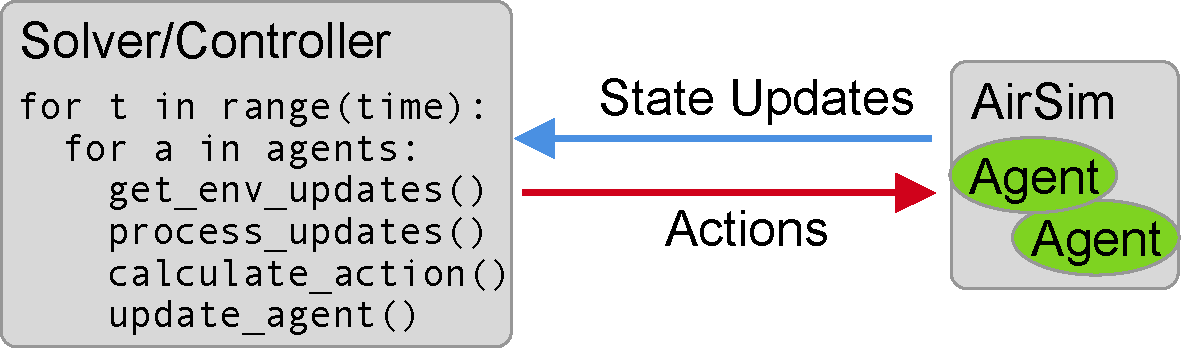
\includegraphics[width=8.31cm]{naive-solver}
	\caption{Example of a simple solver interacting with the simulator.}\label{fig:naive-solver}
\end{figure}

\subsection{Simulator}

This text describes integration with AirSim. AirSim is a simulator for drones, cars and more, built on Unreal Engine. It is open-source, cross platform, and supports hardware-in-loop with popular flight controllers such as PX4 for physically and visually realistic simulations. It is developed as a plugin that can simply be dropped into any Unreal environment \cite{shah2018airsim}. 

\subsection{Akka and Actor Model}
Actor abstraction is a parallel programming model based on actors and messages. Immutable messages are passed between actors asynchronously and delivered into the recipient's mailbox. Each message is then completed in a single threaded fashion. This is also true for the internal state of the actor - it can only be modified and accessed by the actor \cite{scala-Akka-streams}. Actor systems easily express a wide range of computational paradigms, and provide a natural extension of programming into concurrent (parallel) systems. This naturalness and ease of expression means that programs to solve complex problems do not add even more complexity of their own. This direct relationship of the code to the problem domain also makes it easier to optimize algorithms based on knowledge of that domain \cite{actor-foundation}.


\subsubsection{Communication with AirSim}
AirSim uses MessagePack \cite{messagepack} for communication. MessagePack is an RPC (Remote Procedure Call) implementation that provides fast and efficient communication between components written in different languages. At the time of writing, the last update of the JVM implementation depends on a deprecated version of MessagePack serializer\footnote{Version 0.6.6 of MessagePack for Java (https://github.com/msgpack/msgpack-java)}. The RPC implementation doesn't provide any error handling which makes it impossible to properly handle errors returned by AirSim. This implementation cannot be used for camera feed because the images returned by \verb|simGetImage| call exceed the allowed value size. Lastly, mapping between its Value types and native Scala types is either missing or is problematic and slow.  

As such the a custom RPC implementation using a routing pool of Akka TCP clients was used. The solver uses ask messages to to send commands and receive responses in a non-blocking manner. A Scala msgpack4s\footnote{https://github.com/velvia/msgpack4s} library was used for serialization/de-serialization.
%Figure \ref{fig:flow-in} shows how Akka Flow is used to map the vehicle name to the location in a non-blocking manner using the ask pattern.
%\begin{figure}
%	\centering
%	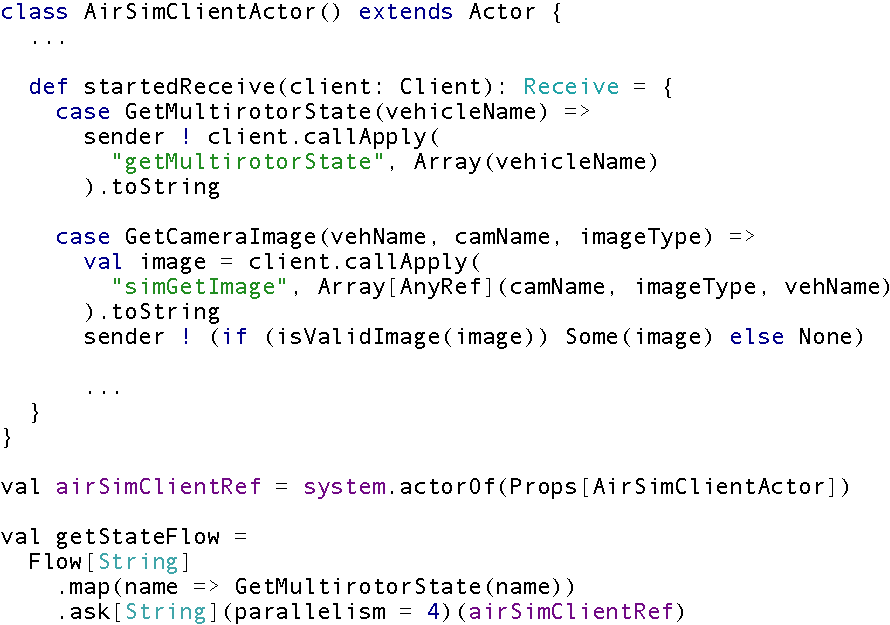
\includegraphics[width=8.6cm]{air-sim-client}
%	\caption{Flow transforming vehicle name to multi-rotor state string.}\label{fig:air-sim-client}
%\end{figure}


%Because multiple components need to interact with AirSim and the interaction is stateless (the only state is the open connection, but each connection can handle any commands from any component), it is a good use-case for Akka routing. Akka Router creates a pool of actors and each of them opens a connection at the start of the simulation. If a component (e.g. position tracker) requires location update, it passes a message to the router. The router then routes the message to the actor. Once the actor receives a response from AirSim, it returns it to the component in the form of message. Because most of the components are Akka Streams and not actors, this call is encapsulated in a \verb|Flow| using the ask pattern. 


%A simplified code is shown in Figure \ref{fig:air-sim-client}. \verb|AirSimClientActor| receives messages such as \verb|GetMultirotorState| or \verb|GetCameraImage|, interacts with the AirSim and returns the result to the sender of the message. Flow \verb|getStateFlow| uses \verb|ask| pattern to interact with the actor. Parallelism argument is related to back pressure. It allows these calls to be parallelized (e.g. if some of the responses take longer to process than the query interval).


\subsection{Reactive Streams}
%On a micro level, the simulation can be seen as a set of steps (query the environment, evaluate the result, decide the next action, send the action to the environment, etc.), however, on the macro level it can be viewed as data flow. There is some data flowing out of the environment (location updates, camera stream, etc.) and some data flowing back in (steering directions). Without the data flow, the system resembles the Figure \ref{fig:before-stream}. The components interact freely to receive the data they need to do their job. If the components are encapsulated as \verb|Actor|s to allow for parallel processing of messages, this represents a workable solution. With growing number of sensor outputs and varying requirements of the solver inputs, however, it becomes difficult to maintain and extend.


High fidelity simulators generate large amount of data that needs to be processed in near real-time. Each agent can generate multiple streams (e.g. location updates, camera feed, LIDAR feed, etc.) and streams from multiple agents may need to combined (e.g. in synchronized movement of multiple vehicles). Each stream may need multiple transformations (e.g. deserialization, conversion, calculations, etc.) and those transformations may need to be parallelized to increase throughput.
Reactive Streams is an initiative to provide a standard for asynchronous stream processing with non-blocking back pressure. This encompasses efforts aimed at runtime environments (JVM and JavaScript) as well as network protocols. \cite{reactive-manifesto} 

\subsubsection{Back pressure}
In a system without back pressure, if the subscriber is slower than the publisher, then eventually the stream will stop - either because one of the parties runs out of memory and one of its buffers overflows or because the implementation can detect this situation but cannot  stop sending or accepting data until the situation is resolved (if it can be resolved at all). Although the latter scenario is somewhat more positive than the former, blocking back pressure (the capability of a system to detect when it must slow down and to do so by blocking) brings with it all of the disadvantages of a blocking system, which occupies resources such as thread and memory usage. \cite{reactive-web-apps}

\subsection{Domain Specific Language (DSL)}
\begin{figure*}
	\centering
	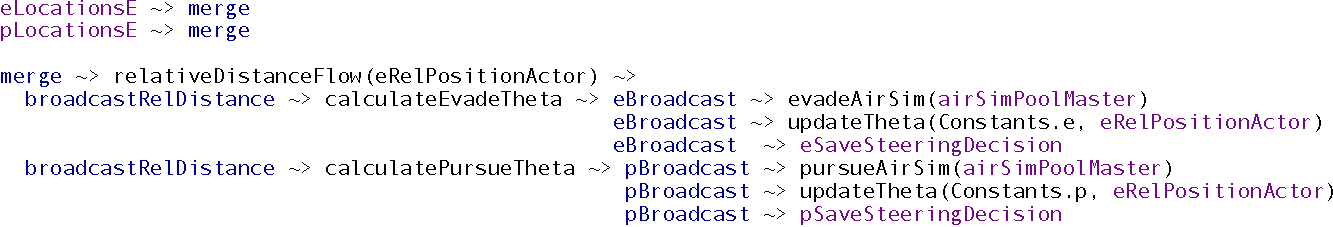
\includegraphics[width=17.0cm]{streams-SDL}
	\caption{The graph controlling the simulation expressed using the Akka Streams DSL. Symbol $\sim$$>$ stands for ``feeds into".}\label{fig:streas-SDL}
\end{figure*}

Besides technical reasons, there is also additional motivation for the reactive streams. They provide a DSL (Domain Specific Language) \cite{dsl-book} to define the stream transformation graphs in a expressive way. In a few lines of code it's very easy to express how the data sources are transformed and how data stream flows between the components and where it's terminated.

This is illustrated in Figure \ref{fig:streas-SDL}. Location streams for both actors are merged together using a merge component and then fed into the relative distance calculator. The result is then broadcast into 2 parallel streams, one for each agent. Based on the relative position, the solver calculates actions in the form of steering thetas. Each steering theta is then broadcast into three parallel streams - the first one to update the AirSim, second to feed the updated theta back to the solver and the last one to persist the steering decision data.





%\begin{figure}
%	\centering
%	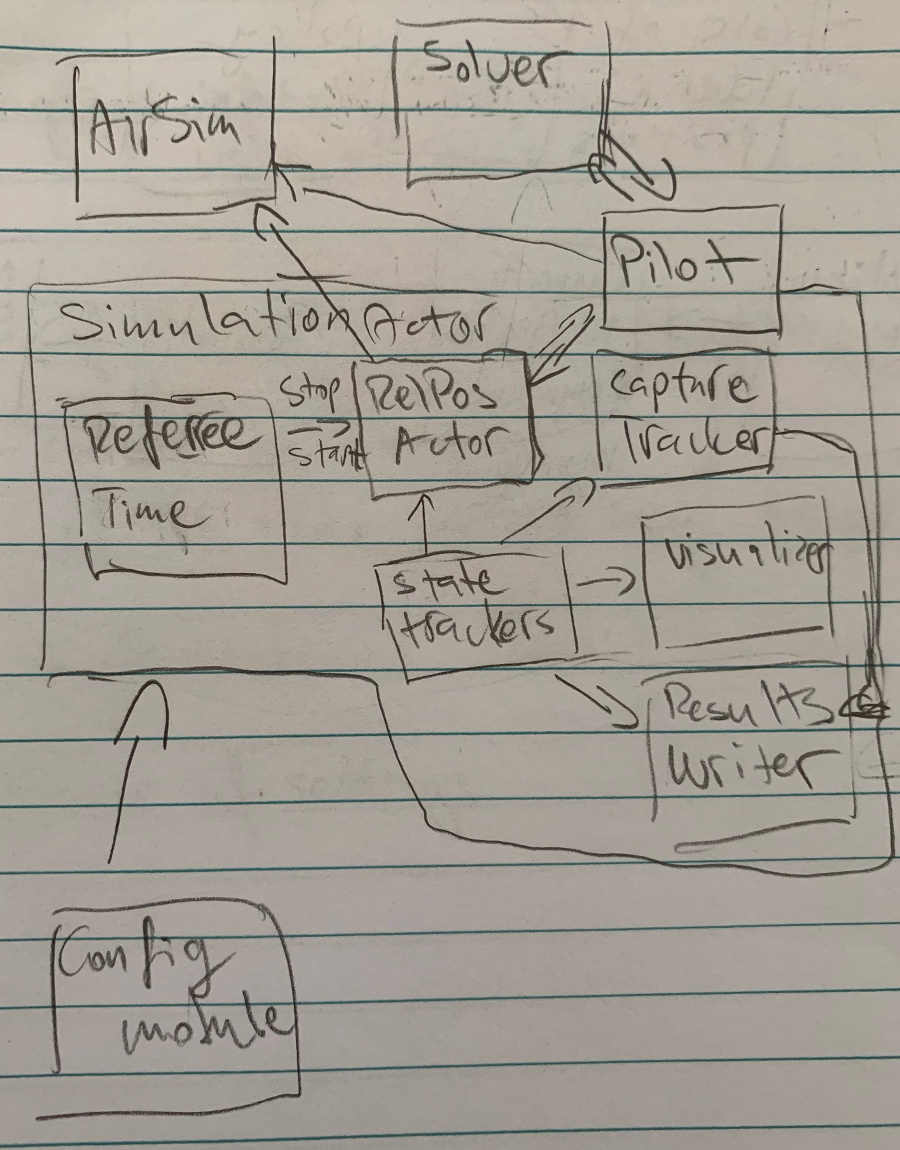
\includegraphics[width=6.0cm]{before-flow}
%	\caption{System design without streams.}\label{fig:before-stream}
%\end{figure}




%\subsection{Message Broker}
%For situation where the solver cannot be implemented in the same program (e.g. because it is implemented in a different programming language) or on the same machine (e.g. because it requires extra resources such as GPU), it is necessary to implement remote messaging.
 
%One way is to use RPC (Remote Procedure Call). There are several options available: AirSim uses MessagePack RPC (Remote Procedure Call), Google uses gRPC for its services, and there are several others. Another option is to use a message broker. The difference is that while RPC calls the remote service directly, with message broker, the services publish and consume messages via the message broker.

%Kafka was developed to collect and distribute massive messages for distributed systems. It is a high-throughput distributed messaging system. Kafka can keep stable performance even if it processes millions of messages per second. \cite{wang2015kafka}

%Figure \ref{fig:after-kafka} shows how such communication works. The raw (or pre-processed) data is published to Kafka (e.g. one topic for location updates, one topic for LIDAR, etc.) and consumed by services that process these data. The results are then published to a different topic. This simplifies dependencies between services, reduces data loss when a service crashes, provides a simplicity of one "API" for communication.



%\begin{figure}
%	\centering
%	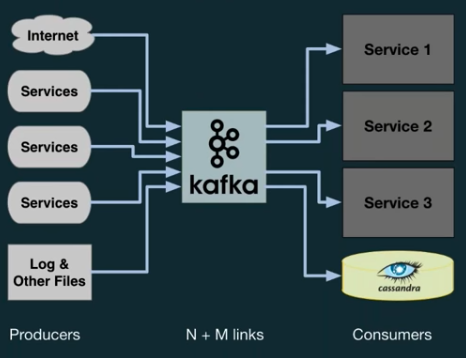
\includegraphics[width=5cm]{after-kafka}
%	\caption{Message broker handles  .}\label{fig:after-kafka}
%\end{figure}


%%%%%%%%%%%%%%%%%%%%%%%%%%%%%%%%%%%%%%%%%%%%%%%%%%%%%%%%%%%%%%%%%%%%%%%%%%%%%%%%
% IMPLEMENTATION
%%%%%%%%%%%%%%%%%%%%%%%%%%%%%%%%%%%%%%%%%%%%%%%%%%%%%%%%%%%%%%%%%%%%%%%%%%%%%%%%
%\section{Implementation}

%\subsection{Akka Streams}
%Figure \ref{fig:with-flow} shows implementation using Akka Streams. Each data flow is encapsulated in the stream. The incoming data is received by a merge/broadcast component that provides a publisher/subscriber functionality. The downstream components subscribe for the input they need (this is transparent to the data producers). Solvers are a special category, because they do not behave as sinks, they behave as flows (i.e. transformations). Solvers transform the input into the output in the form of actions and these actions and then routed through the \verb|AirSimClientActor| back to the AirSim.

%\begin{figure}
%	\centering
%	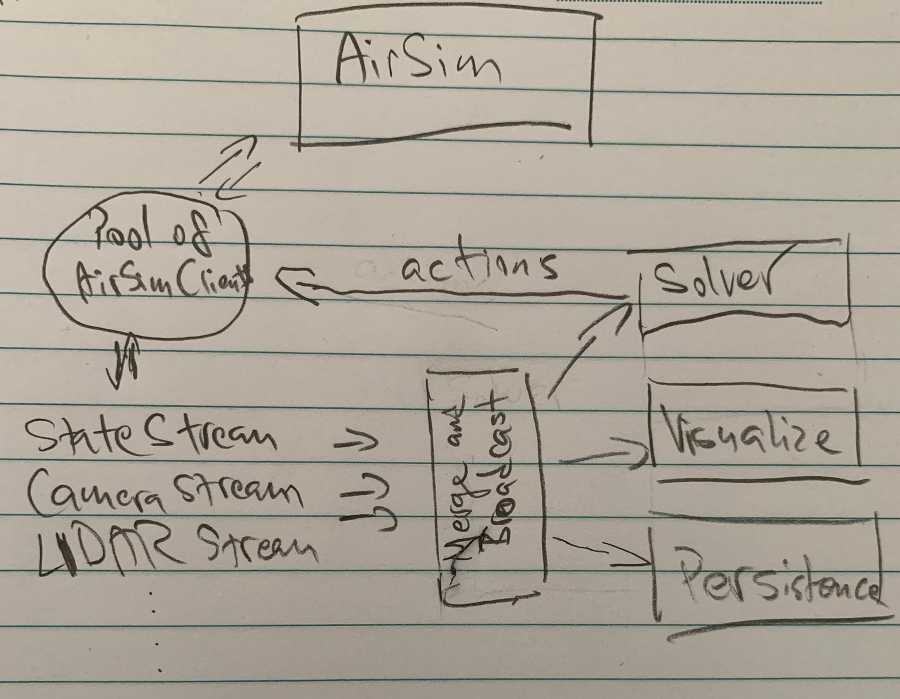
\includegraphics[height=5cm]{with-flow}
%	\caption{Implementation using Akka Streams.}\label{fig:with-flow}
%\end{figure}

% instead show code handling 2 streams and generating a response?
%\begin{figure}
%	\centering
%	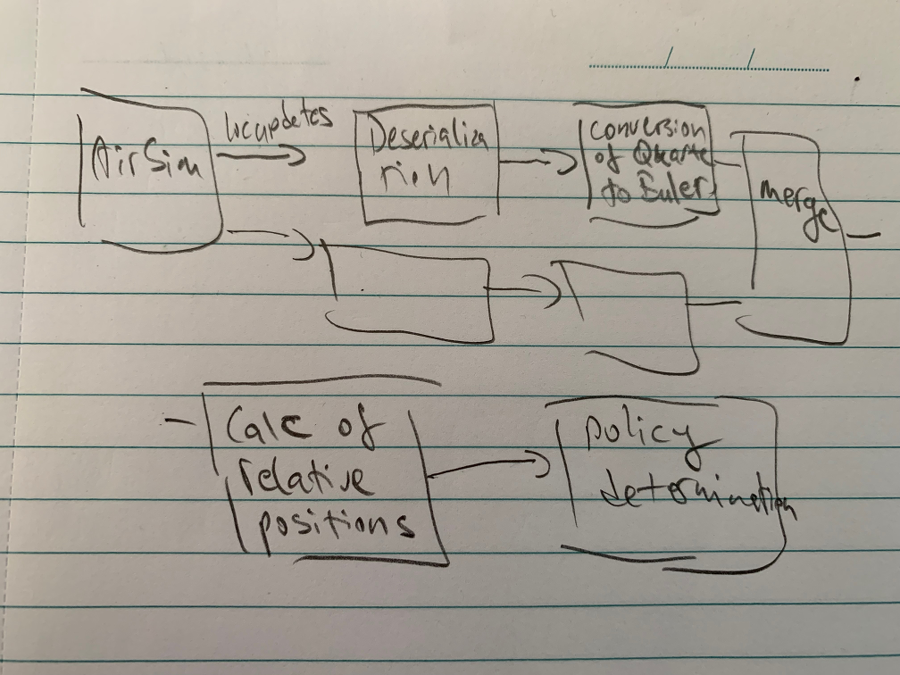
\includegraphics[width=6cm]{flow-in-sketch}
%	\caption{Graph handling location updates stream. Data is received from AirSim, deserialized, converted and fed into the solver that determines the next action.}\label{fig:flow-in}
%\end{figure}

%
%\begin{figure}
%	\centering
%	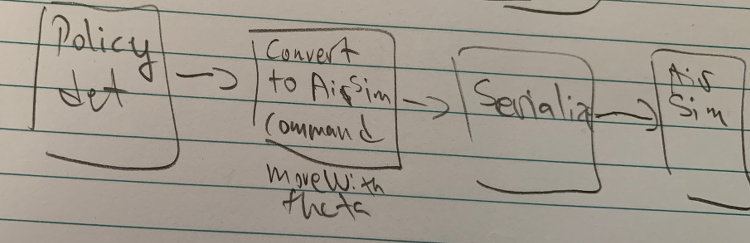
\includegraphics[width=6cm]{flow-out-sketch}
%	\caption{Graph streaming the selected action back to AirSim. The solver returns steering %angle theta that needs to be converted to AirSim command moveByVelocityZ, serialized and sent %to AirSim. }\label{fig:flow-out}
%\end{figure}

%\subsection{Kafka}
%Implementation using Kafka is somewhat similar to the above solution but instead of built-in solver, the streams are terminated in Kafka. Figure \ref{fig:kafka-sink} shows such implementation. These messages are then received by the solver (or any other program), e.g. in Python using \verb|KafkaConsumer|. The solver generates action and this action is then posted back to Kafka on a different topic. Back in the middleware the actions are consumed and using the \verb|AirSimClientActor| routed back to AirSim.

%\begin{figure}
%	\centering
%	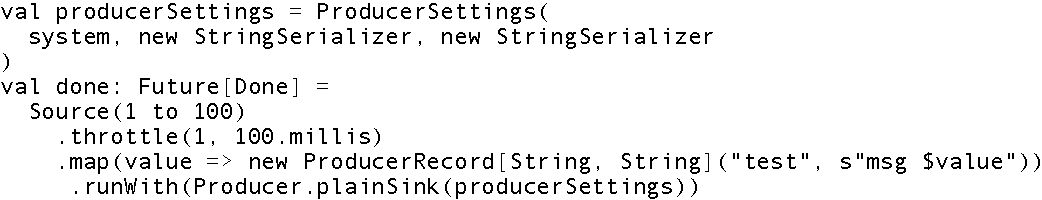
\includegraphics[width=8.3cm]{kafka-sink}
%	\caption{Serializing Akka Stream to Kafka.}\label{fig:kafka-sink}
%\end{figure}


%%%%%%%%%%%%%%%%%%%%%%%%%%%%%%%%%%%%%%%%%%%%%%%%%%%%%%%%%%%%%%%%%%%%%%%%%%%%%%%%
% EXPERIMENTS
%%%%%%%%%%%%%%%%%%%%%%%%%%%%%%%%%%%%%%%%%%%%%%%%%%%%%%%%%%%%%%%%%%%%%%%%%%%%%%%%
\section{Experiments} \label{sec:exp}
The same algorithm was tested in four different setups - sequential model with simulator paused for calculations and communication (this represents the ground truth), sequential model with simulator running throughout, partially parallelized model using futures to encapsulate communication/calculations for each agent at every time step, and fully parallelized model using Akka Streams. Each model was run under 2 different network setups\footnote{The simulator is running on a GPU on GCP (Google Cloud Platform) located in Sydney (zone australia-southeast1) while the solver was located in Brisbane (about 1000km away).}. The first set of experiments was using a direct internet connection which provides stable average latency of 36ms. The second set was run over VPN with average latency of 65ms, fluctuating between 20ms and 200ms (Figure \ref{fig:network-latency} shows the latency details). 

\begin{figure}
	\centering
	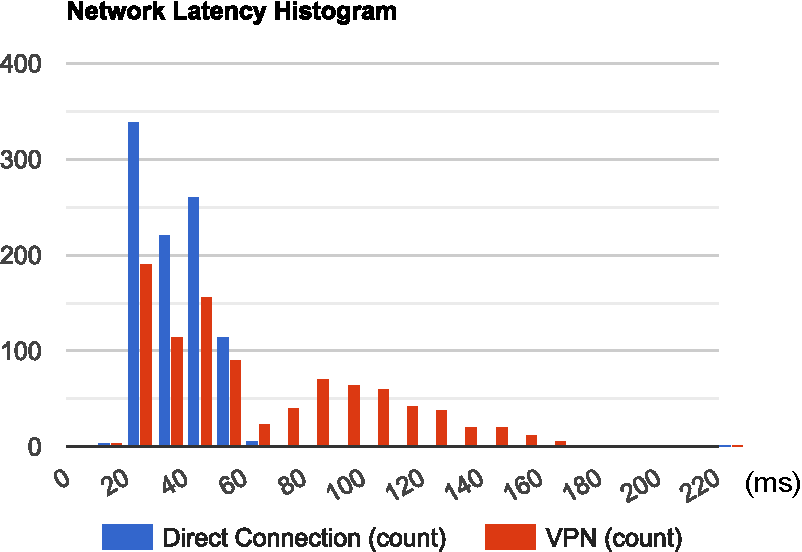
\includegraphics[width=8.0cm]{network-latency}
	\caption{Histogram of the latency using direct connection and VPN.}\label{fig:network-latency}
\end{figure}

Each agent follows a different policy based on models that were originally created for simulation of the differential games \cite{redulla2018simulating}. The pursuer is modeled to intercept the evader and the evader's policy is trying to avoid capture. The pursuer is faster, moving with velocity of 10m/s, but has a larger turning radius of 8m. The evader is slower at velocity of 5m/s, but is more agile and can make turns of any angle. The policy models require position of both players and their headings\footnote{The location data for each player is shared in every implementation to reduce the number of requests because high number of concurrent requests tends to overload AirSim.}. Based on the relative distance, the evader's policy decides if to keep the course or attempt an evasive left or right turn. Pursuer's policy tries to minimize the relative distance by adjusting the heading and speed. This interdependency between the two models make the simulation very sensitive to data flow fluctuations because each model is constantly reacting to the other model (unlike agent flying a predetermined fixed mission).   

Four observations were measured: recency of location data of the player and opponent and time since the last move by the player and opponent.

\subsection{Sequential model with simulator paused between turns}
This represents the ground truth as the paused simulator serves as a synchronization layer that shields the algorithm from both stale data and delays in actions. The simulator starts paused. The measurements are taken, and the actions calculated and sent to the agents. After that, the simulator is run for 100ms. Then the process repeats. Because the communication with the simulator happens in the paused state it can be done in a blocking manner and the calculations start only once all the requests have finished.

\subsection{Sequential model with simulator running}
This is the same as the previous model, but without the paused simulator acting as the synchronization layer. Because all commands run in sequence, the next request can only be sent once the previous one completes and the calculations can only start once all the requests finished. This creates a varying level of staleness among the received data that enter the calculations. It also increases the time lag between actions being sent to the agents. With the pursuer moving at 10m/s, even relatively small delay of 500ms translates to a location difference of 5m.

\subsection{Partially parallelized model}
This model represents a simple (if short-sighted) solution to the concurrency issue. Since each agent is treated as a separate entity, at each timestamp, they are wrapped in their individual future. This means that while all communication and calculations for a single agent runs sequentially, the code blocks for both agents are run in parallel.

\subsection{Fully parallelized model using Akka Streams}
In this model, not only the agents move in parallel, but each operation within each agent is parallelized as well. There are no inter-process dependencies: the location is updated independently, the calculations use whatever latest data available and once the new action is calculated, it is sent to the agent. The whole process moves in the interleaved manner.
%\emph{this whole paragraph needs to be changed}

%\subsection{Fully parallelized model with Kafka - if there's time - definitely no time! }
%This model builds on the previous one and adds on a message broker to allow for out of process and out of machine communication. 

%%%%%%%%%%%%%%%%%%%%%%%%%%%%%%%%%%%%%%%%%%%%%%%%%%%%%%%%%%%%%%%%%%%%%%%%%%%%%%%%
% RESULTS
%%%%%%%%%%%%%%%%%%%%%%%%%%%%%%%%%%%%%%%%%%%%%%%%%%%%%%%%%%%%%%%%%%%%%%%%%%%%%%%%
\section{Results}
Figures \ref{fig:charts-no-vpn} and \ref{fig:charts-vpn} show the summary of the results.  The images represent trajectories generated by pursue flight. The blue color represents the evader and the red color represents the evader. Trajectories in all of the images are using the same algorithm. The first column illustrates the trajectories generated by the agents. Because this is a pursue/evade situation, the distance between the agents is an important measure. This is plotted in the charts in the second column.
Charts in the third column show recency of data used for calculations and time-lag since the last move. Part 1 represents the ground truth. After every step, the simulator was paused for location updates, calculations and communication of actions back to the agents. Parts 2-4 show results without pausing the simulator which caused various degrees of latency, depending on the level of parallelization. Figure \ref{fig:charts-vpn} shows performance of the same algorithm using network connection with higher and much more variable latency.

%%%%%%%%%%%%%%%%%%%%%%%%%%%%%%%%%%%%%%%%%%%%%%%%%%%%%%%%%%%%%%%%%%%%%%%%%%%%%%%%
\begin{figure*}
	\centering
	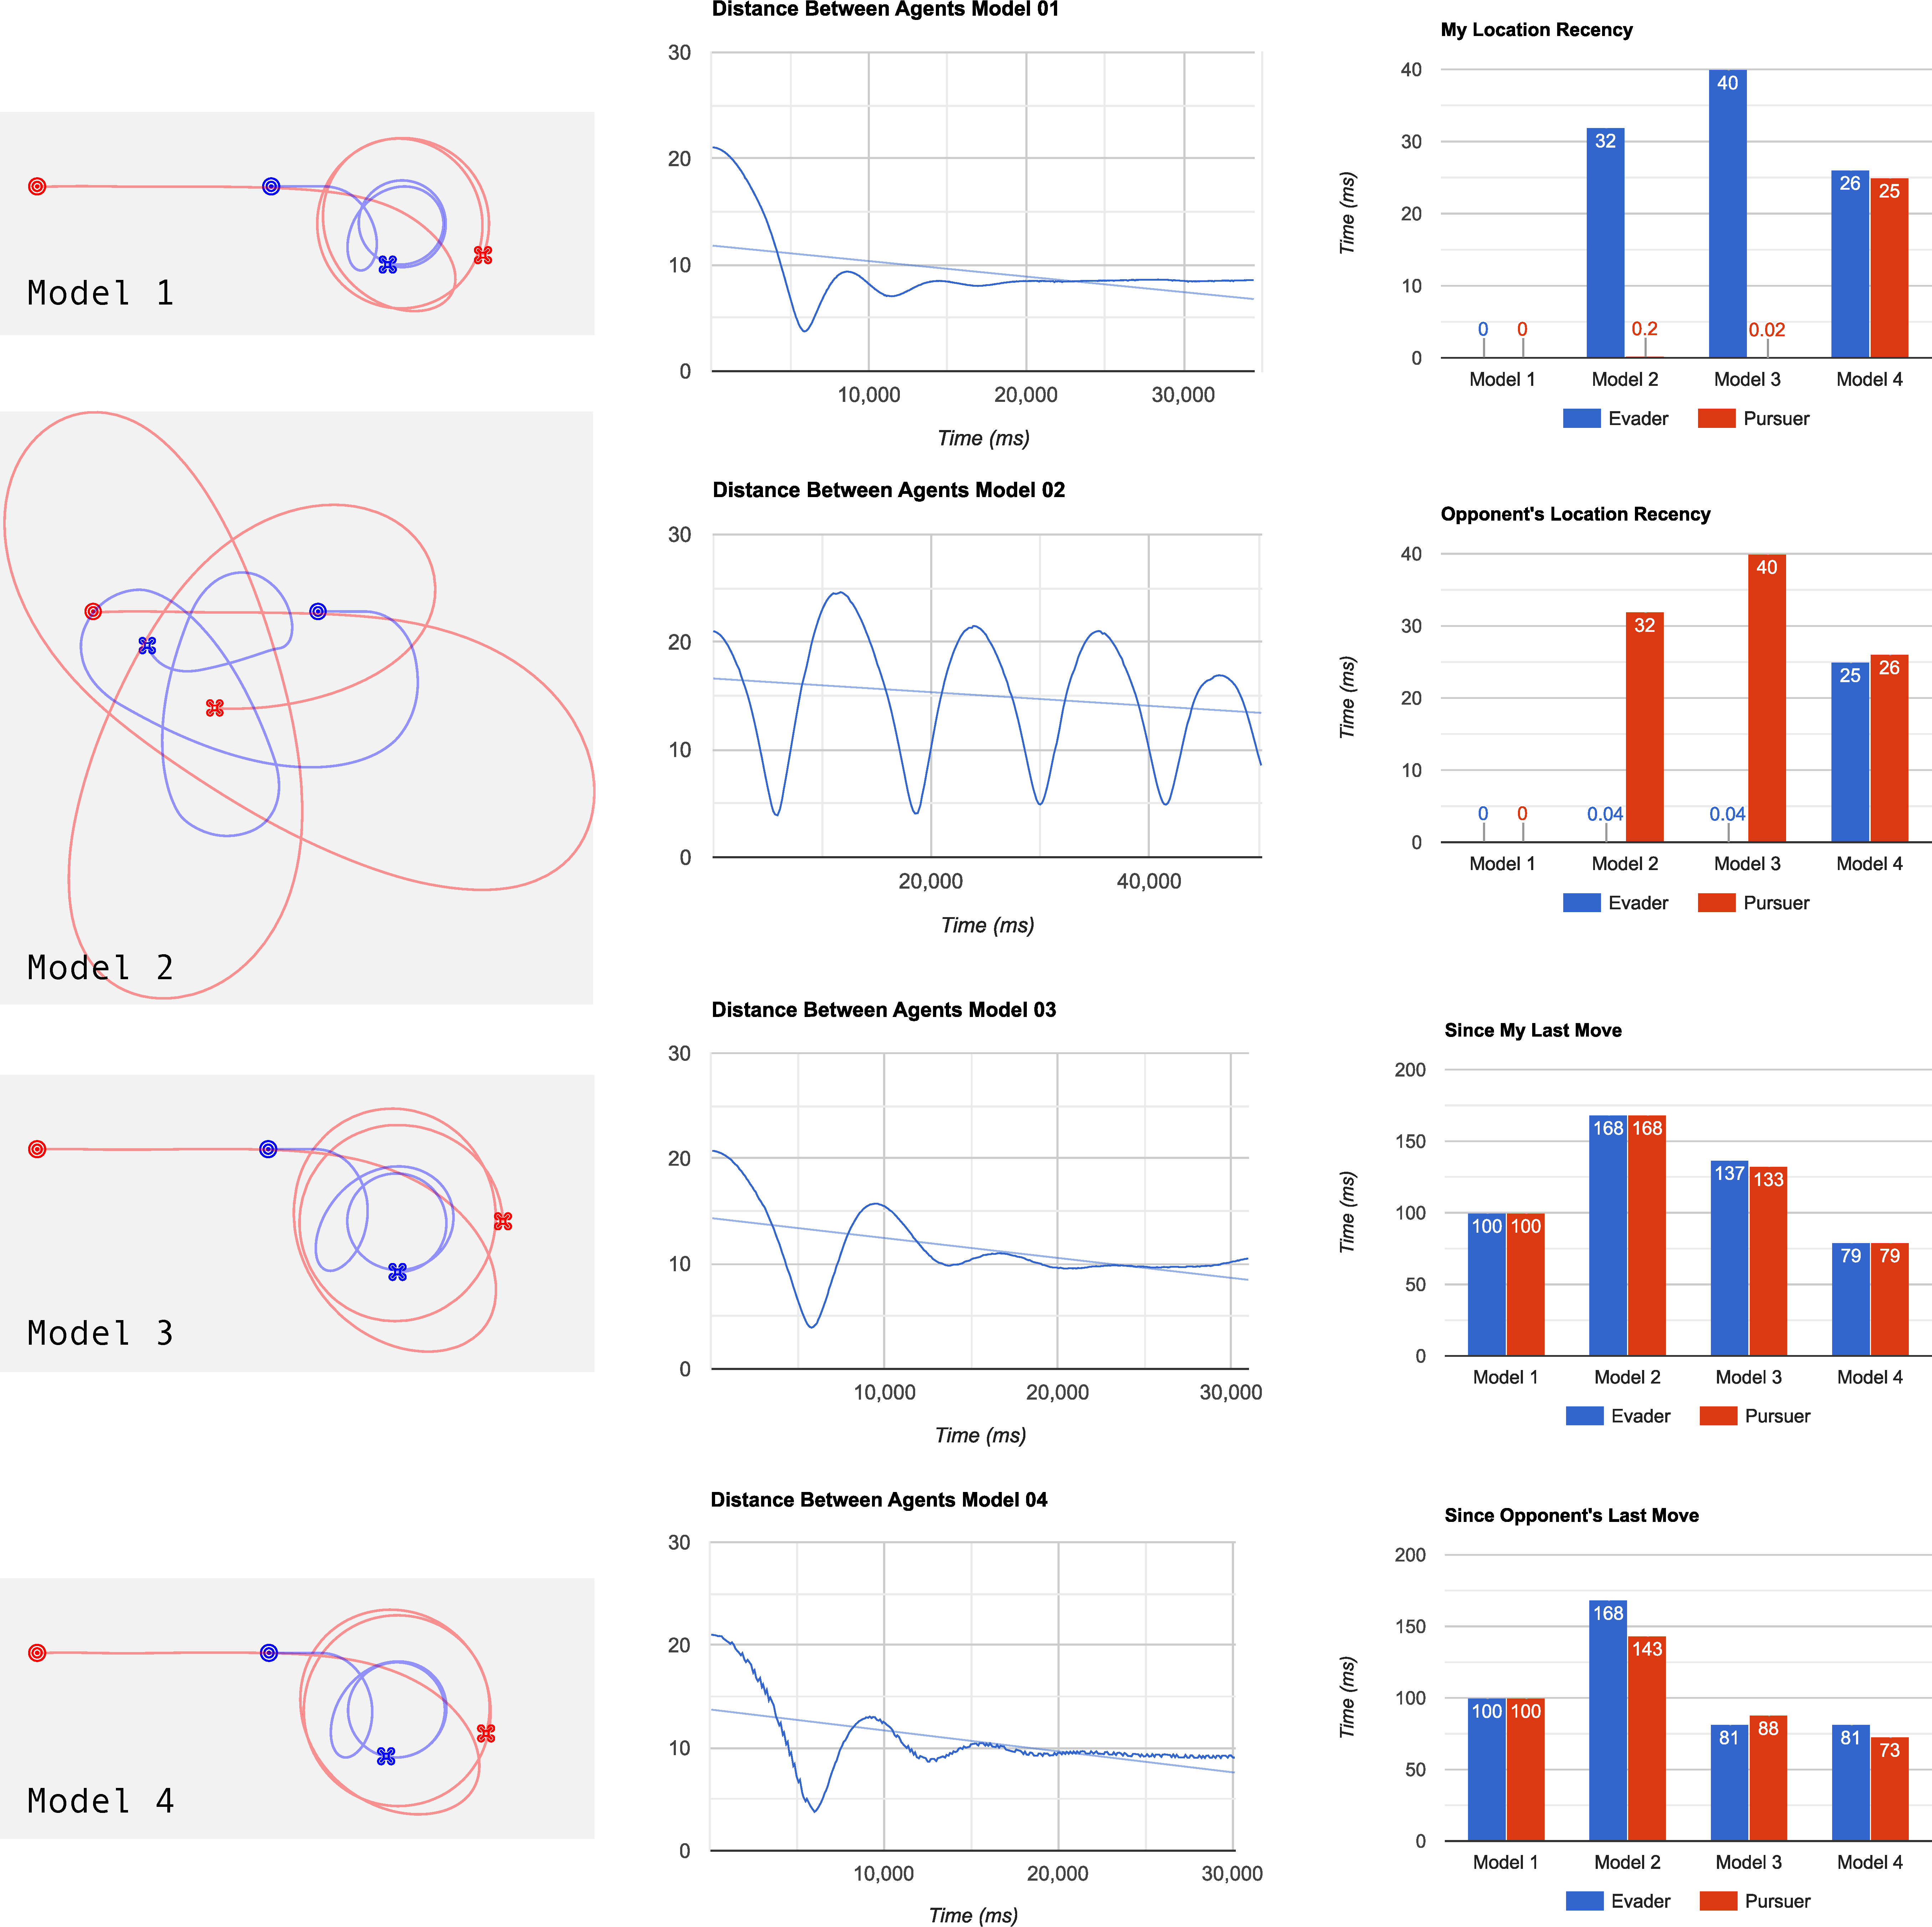
\includegraphics[width=18.0cm]{charts-no-vpn}
	\caption{Results of running the models over a reliable network with latency averaging 36ms. The first column shows the trajectory followed by the agents. The second column shows the distance between the agents. The third column shows the recency of the data used for calculations and delay since the previous step.}\label{fig:charts-no-vpn}
\end{figure*}


\begin{figure*}
	\centering
	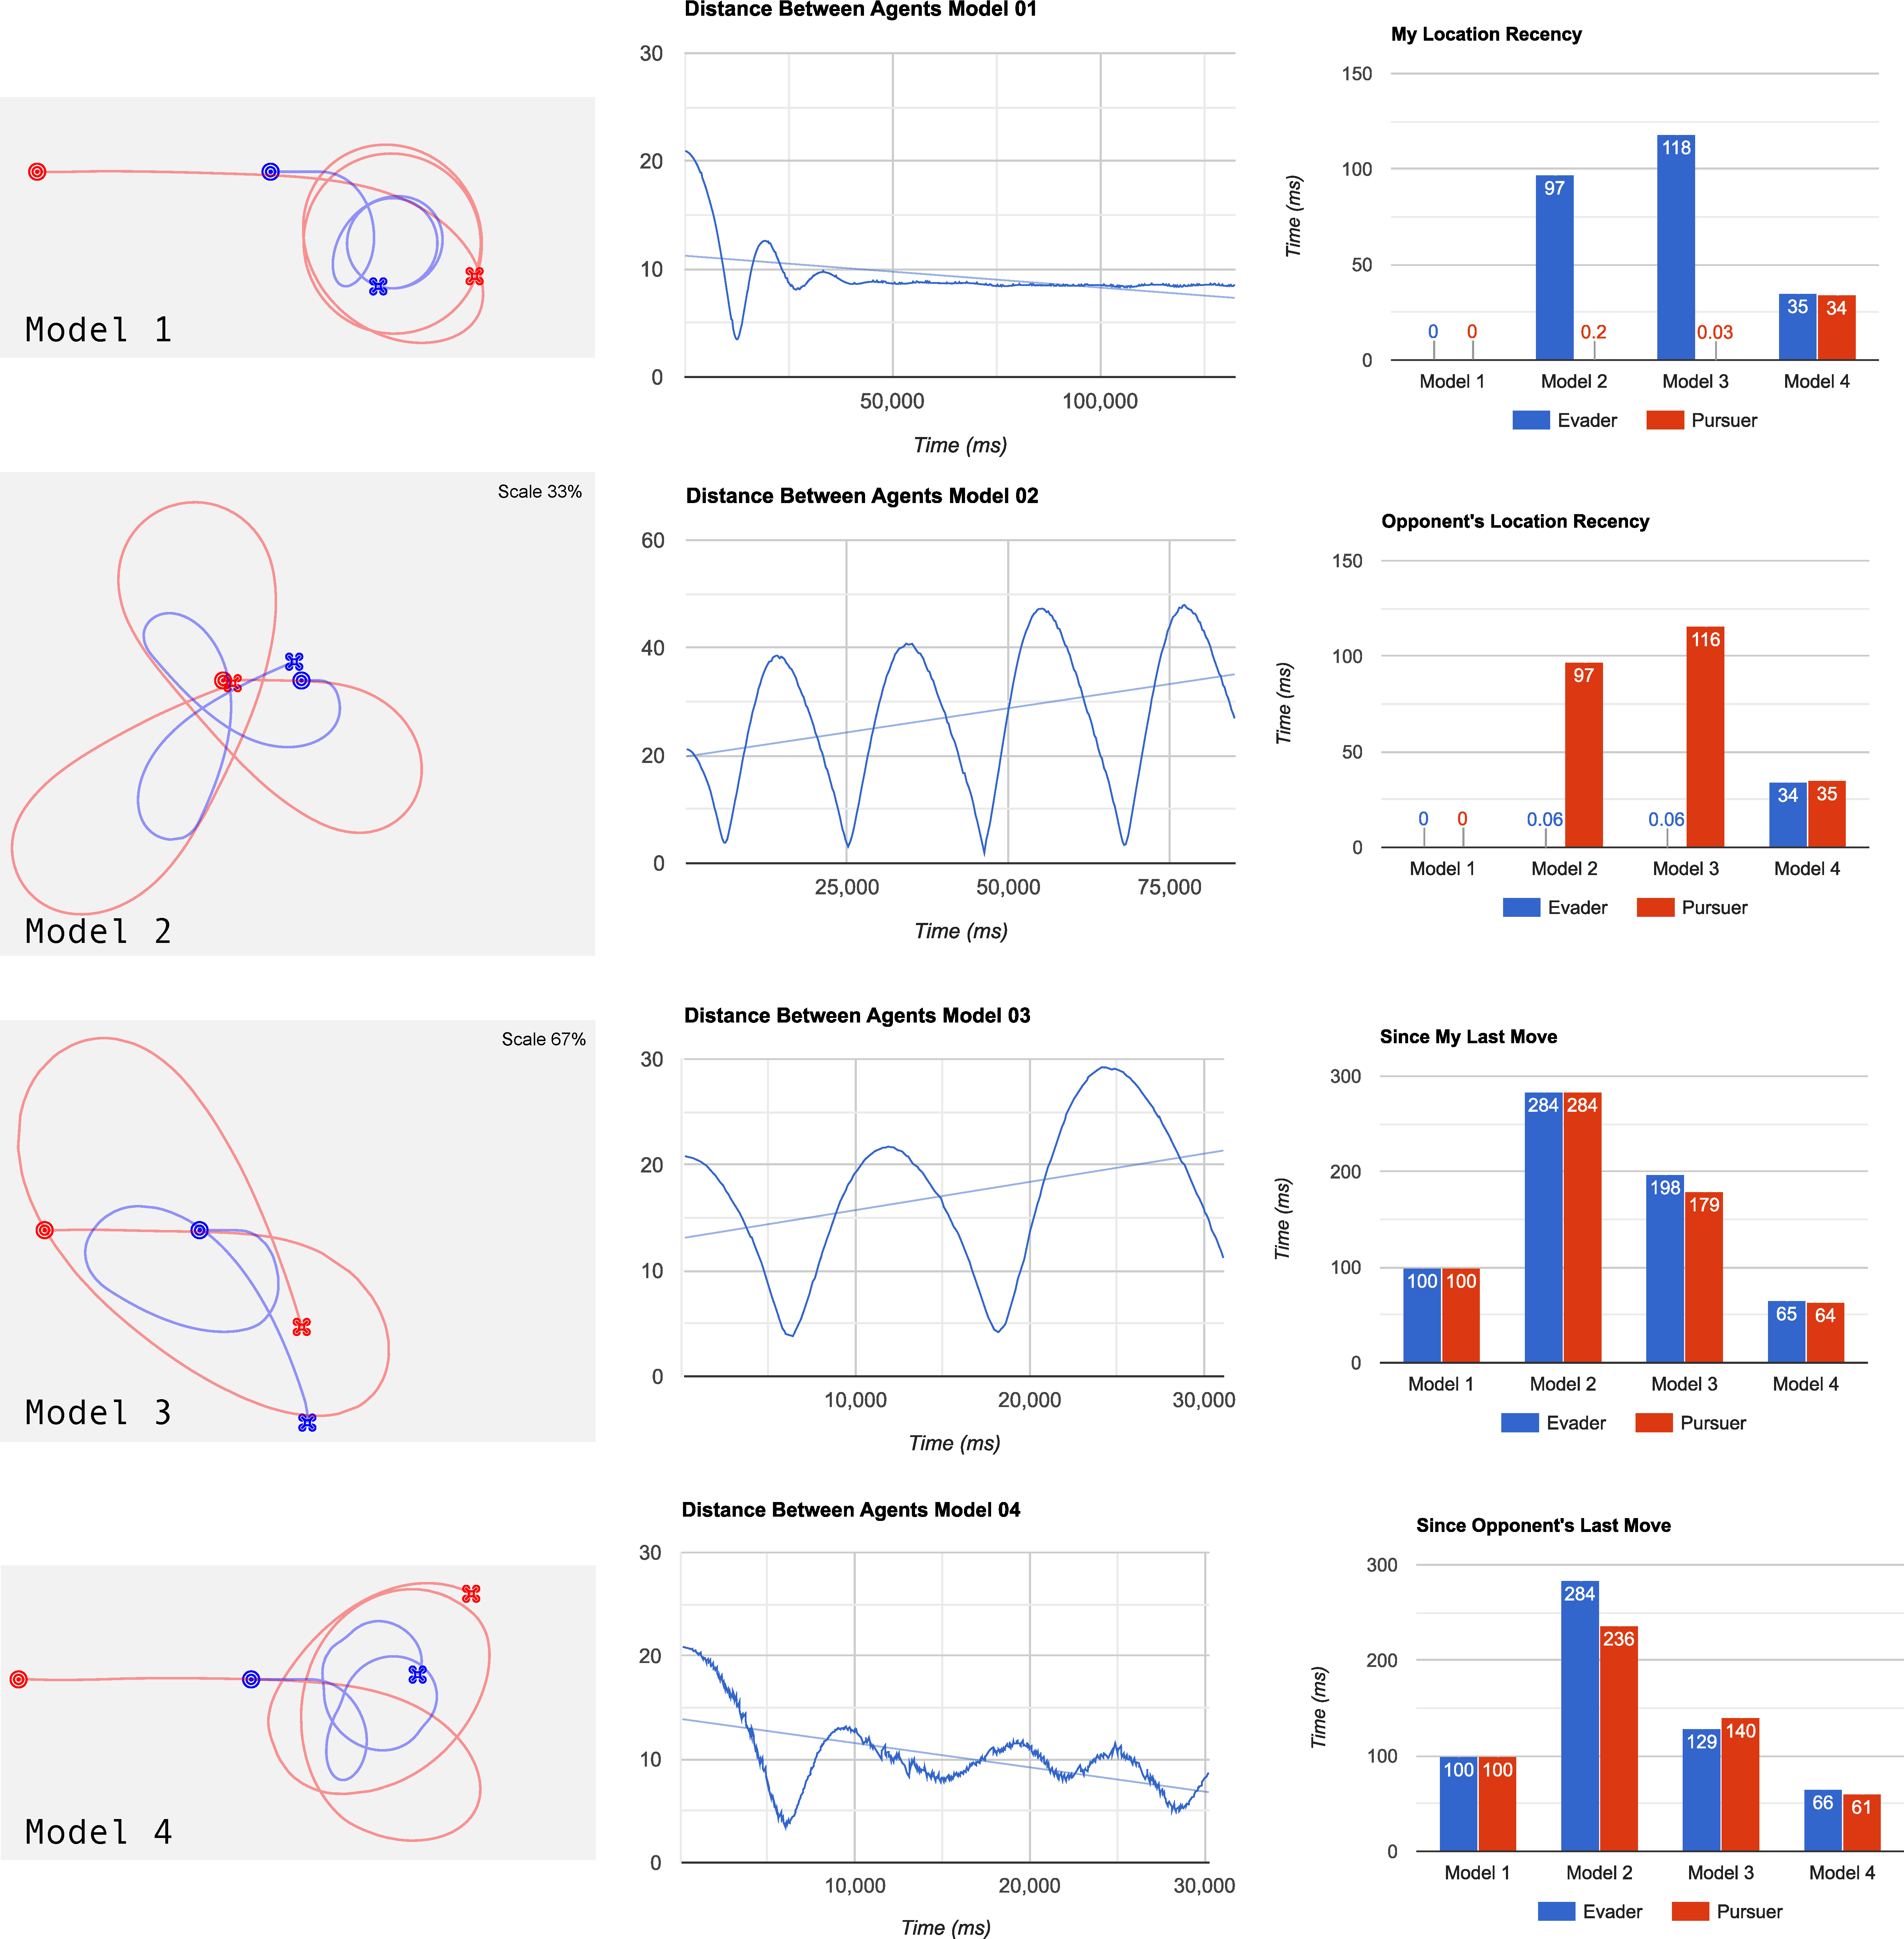
\includegraphics[width=17.0cm]{charts-vpn}
	\caption{Results of running the models over a VPN with fluctuating latency (average of 110ms). The first column shows the trajectory followed by the agents. The second column shows the distance between the agents. The third column shows the recency of the data used for calculations and delay since the previous step.}\label{fig:charts-vpn}
\end{figure*}

%Force the Floats here :-)
\afterpage{\clearpage}
%%%%%%%%%%%%%%%%%%%%%%%%%%%%%%%%%%%%%%%%%%%%%%%%%%%%%%%%%%%%%%%%%%%%%%%%%%%%%%%%

\subsection{Direct Connection}
The first image shows the ground truth with the drones orbiting after about 11s. The distance between the agents converges fast to about 8.55m.

In model 2, the delays caused by the sequential execution of the blocking calls to update location details cause much longer turning times. The effects are more visible in the pursuer's path, because it is moving faster and any delay in control will move it further off course. As a result, the distance is alternating between large and small values.

The partially parallelized model performs well, the trajectory follows the ground truth closely, albeit with a larger diameter. The distance between the agents converges to about 10m. Because both location updates run in parallel, they finish on average in 36ms and the action, sent to back to the simulator, is delayed by the same 36ms as compared to the ground truth (see the Time Since My Last Move chart). This delay causes a minor drift in agents which is what causes the slightly larger radius.

Model 4 follows the ground truth the most closely. The distance converges to 9.1 which results in a slightly more than the ground truth but less than model 3. The delays between moves are very close to 100ms just like in the ground truth model.


\subsection{VPN Connection} 
The sequential model behaves in a similarly to the direct connection, only longer delays cause the agents to drift further away\footnote{The trajectory had to be scaled down 3x to fit display window.}. The relative distance follows the same pattern as before but with larger amplitude. 

When using the direct connection and the partially-parallelized model (model 3), both blocking requests\footnote{The action requests are non-blocking. Each subsequent action cancels the previous task and starts new command.} (location updates for evader and pursuer) finished within the time-step window of 100ms so there were no uncompleted Futures overlapping to future iterations. Under VPN conditions, there are requests taking longer and some of Futures complete in the future iterations. This may lead to actions from older iterations overriding the newer updates and being used instead. Using older data has effects similar to increased latency. Both the trajectory and the relative distance chart are now very similar to the sequential model. The smaller delays cause smaller relative distances.

Fully parallelized model (model 4) performs closest to the ground model. There are visible distortions, however, it does converge to the expected results of orbiting agents.

The cause of the different results is the increased latency and latency fluctuations of the received data and how this latency is propagated through the rest of the system. Model 2 and model 3 do not provide any form of control or management of the latency. In model 2, the rest of the program needs to wait until the request is completed. In model 3, the slower requests don't block the faster requests, but may override them if an earlier and slower request completes on after the faster and later request. It may be tempting to counter this with e.g. lower timeout for the Future and using a sequence data structure to keep the order of Futures, but these only address some of the concerns. What is needed, is a solution able to handle the multiple variable rate data flows concurrently and provide tools, like back pressure to deal with the variable rate.

Using Akka streams, the requests run in parallel, just like in model 3, but the streams provide an order guarantee, which means that results of the requests will be emitted in the same order as they were generated. The timeout of each location update is built-in in the ask pattern and any request taking longer will be skipped transparently to the downstream consumers. The data flow needs to be managed on the other end of the pipe-line as well. Too fast rate of the updates leads to crashes in AirSim. Using streams, this can be achieved through throttle and buffer strategy\footnote{Throttle reduces the rate at which elements are emitted and buffer strategy controls which elements are dropped.}. Using plain Futures, this may be very difficult to achieve.




%%%%%%%%%%%%%%%%%%%%%%%%%%%%%%%%%%%%%%%%%%%%%%%%%%%%%%%%%%%%%%%%%%%%%%%%%%%%%%%%
% CONCLUSION
%%%%%%%%%%%%%%%%%%%%%%%%%%%%%%%%%%%%%%%%%%%%%%%%%%%%%%%%%%%%%%%%%%%%%%%%%%%%%%%%
\section{Conclusion}
We demonstrated the use of Akka Streams to parallelize robot simulation. Extensive forward simulation is important in many approaches used to automatically plan and dynamically control multiple interacting coordinated dynamic robots. The use of parallelized and asynchronous (cloud) simulation systems provides opportunity to distribute the simulation task broadly; however, it also provides the challenge of coordinating and synchronizing the overall process. 
As demonstrated in Parts 2 and 3 of Figures \ref{fig:charts-no-vpn} and  \ref{fig:charts-vpn}, if this is not done carefully the simulation can lead to errant and erratic results. As then shown in Part 4 of Figure \ref{fig:charts-vpn}, the performance of the same algorithm using network connection with higher and much more variable latency can be improved via a streaming architecture.

Akka Streams provide a powerful toolbox for dealing with variable data streams, such as the back pressure to regulate the data flow and encapsulation of data transformations into standalone and reusable components. The complete flow of data from inputs, through transformations to outputs can be described in a simple and expressive DSL. Parallel processing of multiple streams and parallelization within each stream reduces delays resulting from communication with multiple sensors and/or multiple agents as well as delays caused by expensive data processing, such as image recognition or gradient policy updates. 
Effectively dealing with these real-world challenges is necessary when moving from local simulation to distributed simulation systems and further into the real-world applications.

The code developed in order to complete this study is available at {\texttt{\small{https://github.com/RoboticsDesignLab/StreamingSimPaper}}}.

%This is necessary when dealing with multiple inputs from multiple sensors transmitted over the network.  


%
%%==> ADD a REAL CONCLUSION HERE PLEASE :-)  <==
%


%%%%%%%%%%%%%%%%%%%%%%%%%%%%%%%%%%%%%%%%%%%%%%%%%%%%%%%%%%%%%%%%%%%%%%%%%%%%%%%%
%Force the Floats here :-)
%%%%%%%%%%%%%%%%%%%%%%%%%%%%%%%%%%%%%%%%%%%%%%%%%%%%%%%%%%%%%%%%%%%%%%%%%%%%%%%%
\afterpage{\clearpage}

%%%%%%%%%%%%%%%%%%%%%%%%%%%%%%%%%%%%%%%%%%%%%%%%%%%%%%%%%%%%%%%%%%%%%%%%%%%%%%%%
\section*{Acknowledgments}
We acknowledge the Microsoft AirSim open-source project for their simulation tools. %which were part of this paper.
We thank Anne Redulla for discussions and for her open-source simulation and differential game solvers.  This research was partly supported by an Australian Research Council Discovery Project (DP160100714).
%% --> PETER: Feel free to add something here if you want to :-)


%%%%%%%%%%%%%%%%%%%%%%%%%%%%%%%%%%%%%%%%%%%%%%%%%%%%%%%%%%%%%%%%%%%%%%%%%%%%%%%%
%% This section was initially prepared using BibTeX.  The .bbl file was
%% placed here later
%\bibliography{publications}
%\bibliographystyle{named}
%% The file named.bst is a bibliography style file for BibTeX 0.99c
\bibliographystyle{named}
\bibliography{bibfile}



\end{document}
%%%%%%%%%%%%%%%%%%%%%%%%%%%%%%%%%%%%%%%%%%%%%%%%%%%%%%%%%%%%%%%%%%%%%%%%%%%%%%%%
% ...  THE END :-)  ...
%%%%%%%%%%%%%%%%%%%%%%%%%%%%%%%%%%%%%%%%%%%%%%%%%%%%%%%%%%%%%%%%%%%%%%%%%%%%%%%%

